\PassOptionsToPackage{table}{xcolor}
\documentclass[sigplan,10pt]{acmart}

\usepackage{booktabs} % For formal tables

\usepackage[utf8]{inputenc}
\usepackage{fullpage}

\usepackage{graphics}

\usepackage{graphicx}
\usepackage{subcaption}

\usepackage{multirow}

%\usepackage{setspace}
\usepackage{ragged2e}

	\usepackage{soul}

%\usepackage{flushend}

%\usepackage{indentfirst}

\usepackage{amsthm}
\usepackage{amsmath,amssymb}
%\usepackage{mathrsfs}
\usepackage{mathtools}

\theoremstyle{definition}
\newtheorem{prop}{Proposition}[section]


%% Listing related stuff

\usepackage{listings}
\usepackage{courier}            %Required for pretty listings (more dense)


%% EMACS colors for listing:

\usepackage{color}
\definecolor{sh_comment}{rgb}{0.65, 0.00, 0.00 } % red-ish
\definecolor{sh_keyword}{rgb}{0.37, 0.69, 0.69}  % blue-green
\definecolor{sh_string}{rgb}{0.08, 0.69, 0.08} % green


%% This manipulates the listing numbering. It decreases it by one at the point used.
\newcommand*\lstDNumber{\addtocounter{lstnumber}{-1}}

%% Change from Listing->Algorithm
%% \renewcommand\lstlistingname{Algorithm} % Fix listing caption name: Listing -> Algorithm
%% \renewcommand\lstlistlistingname{Algorithms}
%% \def\lstlistingautorefname{Alg.}

%% \renewcommand{\thelstlisting}{\thesection-\arabic{lstlisting}}
%\renewcommand{\thelstlisting}{\arabic{lstlisting}} % Fix listing numbering Algorithm 1.1 -> Algorithm 1.

%% \renewcommand{\labelenumi}{\roman{enumi}.}

\lstset{
float=[*],
language=C,                % choose the language of the code
%% basicstyle=\linespread{0.9}
%% basicstyle=\scriptsize\ttfamily,
 basicstyle={\linespread{0.97} \scriptsize\ttfamily},
 stringstyle=\color{sh_string},
 keywordstyle = \color{sh_keyword}\bfseries,
 commentstyle=\color{sh_comment}\itshape,
numbers=left,                   % where to put the line-numbers
%% numberstyle=\scriptsize,        % the size of the fonts that are used for the line-numbers
numberstyle=\scriptsize,        % the size of the fonts that are used for the line-numbers
stepnumber=1,                   % the step between two line-numbers. If it is 1 each line will be numbered
numbersep=5pt,                  % how far the line-numbers are from the code
backgroundcolor=\color{white},  % choose the background color. You must add \usepackage{color}
showspaces=false,               % show spaces adding particular underscores
showstringspaces=false,         % underline spaces within strings
showtabs=false,                 % show tabs within strings adding particular underscores
xleftmargin=2em,                % Left margin
frame=lines,                   % adds a frame around the code. none|leftline|topline|bottomline|lines|single|shadowbox
framexleftmargin=1.5em,         % Margin from frame to line numbers
framexbottommargin=0em,         % Distance from last text to frame
morekeywords={in,true,false,and,or,set,is,not},
%% prebreak=\mbox{\tiny$\searrow$},
prebreak=\space,                % Line break: insert this character at the end of the top line
%% postbreak=\mbox{{\color{blue}\scriptsize$\hookrightarrow$}}, % Line break: blue arrow at the beginning of the bottom line
postbreak=\mbox{{\color{blue}\scriptsize$\hookrightarrow$}}, % Line break: blue arrow at the beginning of the bottom line
breaklines=true,                % sets automatic line breaking
breakatwhitespace=false,        % sets if automatic breaks should only happen at whitespace
tabsize=2,                      % sets default tabsize to 2 spaces
captionpos=b,                   % sets the caption-position to top
escapeinside={\@}{\@}             % Escape sequence \@ESCAPED STUFF\@
}

\usepackage{nasm/lang}
\usepackage{nasm/style}
\usepackage{llvm/lang}


% Copyright
\setcopyright{none}
%\setcopyright{acmcopyright}
%\setcopyright{acmlicensed}
%\setcopyright{rightsretained}
%\setcopyright{usgov}
%\setcopyright{usgovmixed}
%\setcopyright{cagov}
%\setcopyright{cagovmixed}


% DOI
%\acmDOI{10.475/123_4}

% ISBN
%\acmISBN{123-4567-24-567/08/06}

%Conference
\acmConference[CGO'18]{International Symposium on
Code Generation and Optimization}{2018}{} 
%\acmYear{1997}
%\copyrightyear{2016}
%
%\acmPrice{15.00}


\newcommand{\etal}{et~al.}

\newcommand{\itercomp}{{iterative compilation}}
\newcommand{\Itercomp}{{Iterative compilation}}
\newcommand{\IterComp}{{Iterative Compilation}}

\newcommand{\flagstype}{\usefont{T1}{cmr}{m}{n}}

\begin{document}
\title{Online {\IterComp}\\Guided by Low Overhead Profiling}
%\titlenote{...}
%\subtitle{...}
%\subtitlenote{...}

\author{ \vspace{10em} }
\affiliation{%
  \institution{ }
}
\email{ }

%\author{Rodrigo C. O. Rocha}
%\affiliation{%
%  \institution{University of Edinburgh, UK}
%}
%\email{r.rocha@ed.ac.uk}

%\author{Pavlos Petoumenos}
%\affiliation{%
%  \institution{University of Edinburgh, UK}
%}
%\email{ppetoume@inf.ed.ac.uk}

%\author{Lu\'is F. W. G\'oes}
%\affiliation{%
%  \institution{PUC Minas, Brazil}
%}
%\email{lfwgoes@pucminas.br}

%\author{Murray Cole}
%\affiliation{
%  \institution{University of Edinburgh, UK}
%}
%\email{mic@inf.ed.ac.uk}

%\author{Zheng Wang}
%\affiliation{%
%  \institution{Lancaster University, UK}
%}
%\email{z.wang@lancaster.ac.uk}

%\author{Hugh Leather}
%\affiliation{%
%  \institution{University of Edinburgh, UK}
%}
%\email{hleather@inf.ed.ac.uk}

\renewcommand{\shortauthors}{R. Rocha et al.}

\begin{abstract}
Efficiently selecting the best combination of compiler optimisations for a program
remains an open problem due to their complex interaction and the large optimisation search space.
{\Itercomp} techniques, which consist of iterating
over this large space searching for the best optimisation,
has the ability to adapt to new platforms, programs and workload while still
having a systematic and simple optimisation process.
Although some recent work have studied the impact of using multiple
input datasets for performing \itercomp, applying this
technique in an online scenario still poses some challenges.

In this paper, our main goal is to enable \itercomp in
online scenarios with the restriction of executing distinct inputs
only once.
In order to address this challenge,
we propose a the use of a work-based metric that allows for comparing different
combination of compiler optimisations even when executed with distinct inputs.
Because of its online nature, we also propose a relaxed instrumentation
that performs low overhead profiling of the amount of work executed, while
being able to trade-off between accuracy and overhead in a controlled manner.
\end{abstract}

%
% The code below should be generated by the tool at
% http://dl.acm.org/ccs.cfm
% Please copy and paste the code instead of the example below. 
%
\begin{CCSXML}
<ccs2012>
<concept>
<concept_id>10011007.10011006.10011041</concept_id>
<concept_desc>Software and its engineering~Compilers</concept_desc>
<concept_significance>500</concept_significance>
</concept>
<concept>
<concept_id>10011007.10011006.10011041.10011043</concept_id>
<concept_desc>Software and its engineering~Retargetable compilers</concept_desc>
<concept_significance>500</concept_significance>
</concept>
</ccs2012>
\end{CCSXML}

%\ccsdesc[500]{Software and its engineering~Compilers}
%\ccsdesc[500]{Software and its engineering~Retargetable compilers}


\keywords{{\IterComp}, Profiling, Relaxed Instrumentation}

\maketitle

\section{Introduction}

Modern optimising compilers have reached a high level of sophistication, providing a large number of optimisations.
Because of the unpredictability of optimisation interactions, in addition to the growing complexity of processor architectures and applications, the correct choice of optimisations and their ordering can have a significant impact on the performance of the code being optimised~\cite{pan06,fursin07,kulkarni12}.

Each of these optimisations interacts with the code in complicated ways, depending on all other optimisations and the order they were applied to the code being optimised.
Understanding the interactions of optimisations is very important in determining a good solution to the phase-ordering problem~\cite{touati06,kulkarni12}.
Because of all those dependencies and interactions, although most compiler optimisations yield significant improvements in many programs, the potential for performance degradation in certain program patterns is known to compiler writers and many users~\cite{pan06,zhou12,kulkarni12}.
%Traditional compilers typically apply the same set of optimisation in a fixed order to all functions in a program, without regard the code being optimised.

Efficiently selecting the best combination of compiler optimisations for a given program or program section remains an open problem.
Compiler writers typically use a combination of experience and insight to construct the default sequences of prearranged optimisations found in compilers.
However, these default pre-arranged set of optimisations do not include all possible optimisations and they are always applied in the same pre-defined fixed order, without regard the code being optimised~\cite{pan06,cavazos07,zhou12,kulkarni12}.
%in hopes that a programmer will know which combination of optimisations will benefit their code~\cite{pan06,cavazos07,zhou12,kulkarni12}.

A well known compilation technique that addresses this challenge is {\itercomp}.
{\Itercomp} has the ability to adapt to new platforms, program and workload while still having a systematic and simple optimisation process.
It works by repeatedly evaluating a large number of compiler optimisations until the best combination is found for a particular program~\cite{fursin07,chen10}.
The main challenge concerning {\itercomp} is the need for efficiently exploring such a large optimisation space~\cite{fursin07,cavazos07,zhou12}.

Until recently, most of existing work  had been focusing on finding the best optimisation through repeated runs using a single input.
Although they demonstrate the potential of {\itercomp}, in real scenarios the user rarely executes the same input dataset multiple times~\cite{bodin98,kisuki99,stephenson03,kulkarni04,agakov06}.
Applying {\itercomp} in light of a single input may not result in good performance when executing the optimised code with different inputs.

Most of real world applications are complex enough so that a single input case does not capture the whole range of possible scenarios and program behaviour~\cite{haneda06,fursin07,chen10,chen12a}.
Because programs can exhibit behaviours that differ greatly depending on the input,
%This is something that is well known when writing test cases for correctness.
%We can extend the same argument when optimising the code for performance.
using a single input for {\itercomp} can produce poor performance when executed with different inputs.

Recent work have been studying the impact of using multiple input datasets
for performing {\itercomp}.
This previous work suggests that optimising based on a representative range of input datasets allows for selecting a robust compiler optimisation that produces good performance in real scenarios where the input is expected to change constantly~\cite{haneda06,fursin07,chen10,chen12a,chen12b,fang15,mpeis16}.
Their results show that a limited number of input datasets may be sufficient to obtain a well optimised program for a wider range of different inputs~\cite{haneda06,fursin07,chen10,chen12a}.

Finding such a robust combination of compiler optimisations by means of {\itercomp} across a large range of inputs may be very time consuming.
In order to speed up this process we intend to reduce the number of actual executions during the exploration of the optimisation space without much degradation of the final selected optimisation.

\begin{figure}[htb]
    \centering
    \includegraphics[width=\linewidth]{figs/infra-diagram}
    \caption{Overview of the execution engine for applying {\itercomp}.}
    \label{fig:infra-diagram}
\end{figure}

In this paper, our main goal is to enable {\itercomp} in \textit{online} scenarios with the restriction of executing distinct inputs only once, while targeting optimal performance across different inputs.
This online aspect is usually found in mobile and data centre platforms~\cite{chen12b,fang15,mpeis16}, where the goal is to optimise programs based on the workload of a particular user (or group of users) between executions.

Measuring just execution time, for example, is useful only if the amount of work is constant between executions with different inputs.
For this reason, we propose the use of a work-based metric in order to compare the performance of different optimisations across multiple executions of the program with distinct inputs.

Because of the restriction of not repeating inputs, we instrument the program for measuring the amount of work it performed during its execution.
Having a low overhead instrumentation is essential in this online scenario for two main reasons:
$(i)$ the user is directly affected by large overheads;
$(ii)$ a highly intrusive instrumentation can havea significant impact on the effect of the optimisations.

Our main contributions are the following:
\begin{itemize}
\item The use of a work-based performance metric in order to enable \textit{online} {\itercomp} by comparing different combination of compiler optimisations even when executed with distinct inputs.
\item We propose a relaxed instrumentation for low overhead profiling, with a controlled trade-off between accuracy and overhead.
\end{itemize}

\section{Work-based Metric} \label{sec:metric}

In this section we define the work-based performance (WP) metric proposed for comparing different optimised versions of a program when executing with different inputs.
We define the performance metric as the ratio between the amount of \textit{work}, $\Delta W$, performed during a period of time, $\Delta t$.
\[
   P = \frac{\Delta W}{\Delta t}
\]

%The hypothesis is that, given two optimisations $o_1$ and $o_2$, a program compiled with optimisation $o_2$ would \textit{consistently} perform better than when it is compiled with $o_1$, i.e., $o_1 \tilde{<}_p \, o_2$, if it performs more \textit{work} per unit of time when compiled with $o_2$ instead of $o_1$. 
By measuring the amount of \textit{work} done per unit of time, we reduce the impact of input-dependent aspects and focus instead on the efficiency of the optimised program.
For this metric, the main challenge is to precisely define what represents \textit{work}.
As discussed in Section~\ref{sec:related-metrics}, many work metrics have been presented in the literature, such as block frequency and others.
However, for comparing the performance benefits of different compiler optimisations on a program, although block frequency would be able to capture aspects of optimisations that simplify the control-flow graph (CFG), we argue that measuring work only at the basic block resolution would not be enough for capturing the effects of optimisations at the instruction level.
For this reason, we extend the idea of using basic block frequency to measure computational work by also considering the computational cost of each basic block.

%For that purpose, we intend to use profiling techniques to measure the input size and amount of computation performed on the execution path triggered by the input~\cite{ball94,ball96,zaparanuks12,coppa14}.
%In addition to being useful for speeding up {\itercomp} across a large number of different inputs, this metric based on comparing work-based efficiencies could
%potentially be used for applying {\itercomp} \textit{online}.
%However, the overhead for estimating the amount of \textit{work} must be low enough for the performance gains to be beneficial.
To this end, we model the computational work $\Delta W$ as a linear equation based on block frequency information and a cost model of the instruction set.
Formally,
\[
\Delta W = \varepsilon + \sum_{B} w(B)f(B)
\]
where $f(B)$ represents the frequency of basic block $B$ and $w(B)$ represents the computational work of executing $B$.
We define the work of a basic block $B$ as the sum of the cost of its instructions, i.e.,
\[
w(B) = \sum_{i} w_i N_B(i)
\]
where $w_i$ is the cost of instruction $i$ and $N_B(i)$ is the number of occurrences of instruction $i$ in basic block $B$.

In this simplified model, we consider that $w_i$ is constant across all programs and executions, varying only between target architectures.
On the other hand, $N_B(i)$ is a program-dependent static value which is known at compile-time and $f(B)$ is a dynamic value known only at run-time,
since $f(B)$ is both program and execution dependent as the execution frequency of a basic block can change when executing with different inputs.
%However, $N_B(i)$ is program dependent but constant across executions, while $f(B)$ is both program and execution dependent, since $f(B)$ can change when executing with different inputs.
%In other words, $N_B(i)$ is a static value known at compile-time and $f(B)$ is a dynamic value known only at run-time.

%If we define $x_i$ as
%\[
%x_i = \sum_{B\in P} N_B(i)f(B)
%\]
%we can write our definition of work $\Delta W$ as the following linear equation
%\[
%\Delta W = \varepsilon + \sum_{i\in I} w_i x_i
%\]

%\subsection{Linear regression}
%
%\begin{figure}[htb]
%    \centering
%    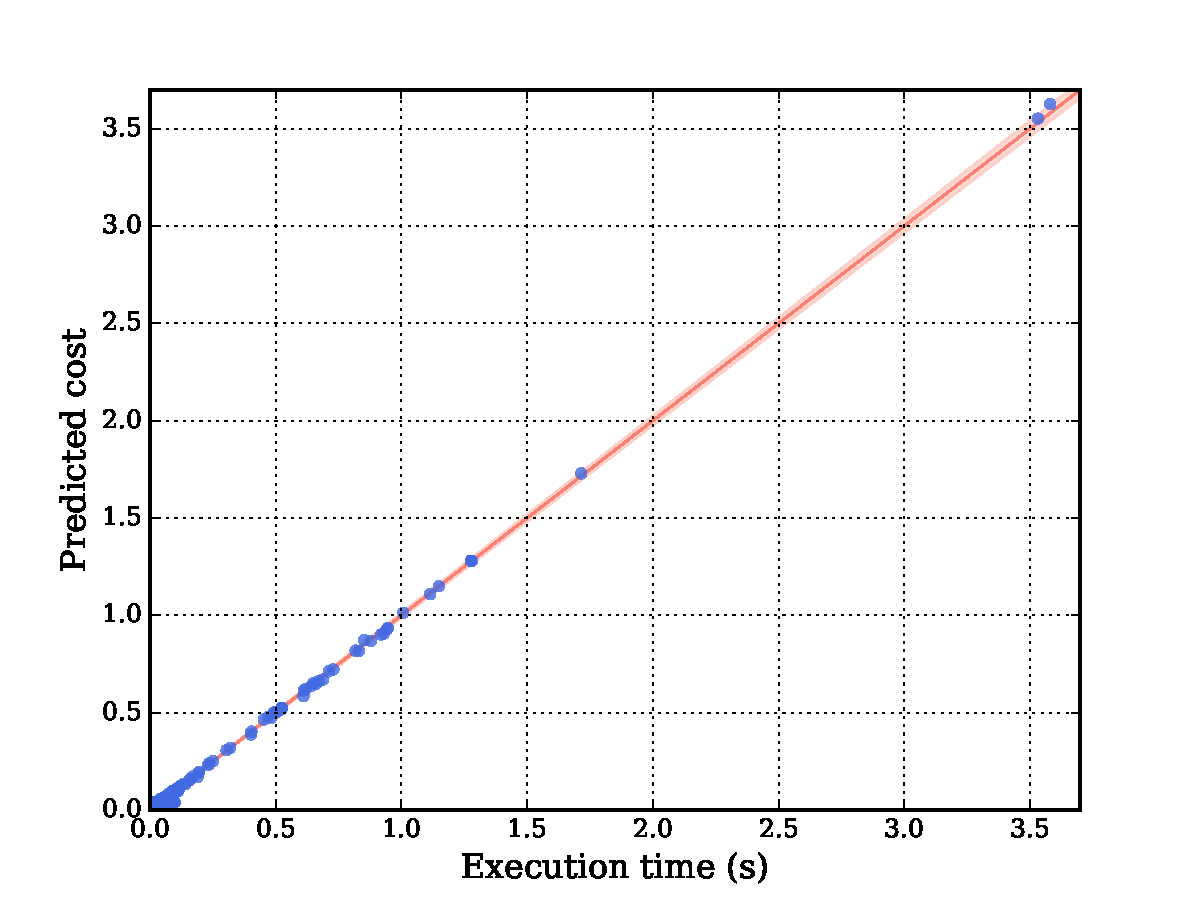
\includegraphics[width=\linewidth]{figs/cost-model.pdf}
%    \caption{Comparison between the naive and optimal instrumentation with no compiler optimisation.} %, i.e., compiled with \textbf{\texttt{-O0}}.}
%    \label{fig:cost-model}
%\end{figure}
%mse 0.000145373168444
%mae 0.00737261168981
%mae* 0.0033892281406
%mape 75.2924320971
%corr (0.99946441743545622, 0.0)

\subsection{Estimating a Cost Model of the Instructions}

Similarly to previous work~\citep{giusto01,powell09,brandolese11}, we derive the cost model of the instruction set by modelling the problem as a multi-variable linear regression, where the \textit{regression coefficients} are the costs of the instructions and the \textit{regressors} are computed as $\sum_B N_B(i)f(B)$ for each instruction.
\begin{equation}\label{eq:linear-work-expression}
\Delta W = \varepsilon + \sum_{i} \left(w_i \sum_{B} N_B(i)f(B)\right)
\end{equation}
By having some empirical data after executing several benchmarks with different inputs, we can fit the linear model with this empirical data in order to obtain estimate costs of the instructions.
In order to fit the linear model, we measure the wall-clock time when executing the training benchmarks described in Section\ref{sec:benchmarks} with their respective 1000 input datasets.
For these measurements, the training benchmarks are compiled without optimisation.
The reason for using no optimisation, as discussed in Section\ref{sec:oic-infra}, is because the amount of work must be only input dependent and consistent between different optimisation sequences.
This aspect is crucial for the work-based performance metric to enable a consistent comparison between the various optimisation sequences when executing with distinct inputs.
%it allows to use the estimated cost model for computing a work metric which is independent of optimisations, as we explained in Section~\ref{}.

Our cost model has a total of 52 LLVM instructions\footnote{We do not model all LLVM instructions because some instructions are more common in optimised programs, such as the vector instructions.}.
Every program, in the set of training benchmarks, was compiled twice: once including the necessary instrumentation for the block frequency profiling, which is required for deriving the linear expression defined in Equation~\ref{eq:linear-work-expression};
and a standard compilation without any optimisation or instrumentation.
For each input in the training dataset, the benchmarks were executed once with the instrumented version for collecting the block frequency profiling, and multiple times with the standard compilation just for measuring the wall-clock execution time, until the confidence interval was no larger than 1\% for a 99\% confidence.
After collecting these measurements, this data can be used to estimate the unknown parameters in the linear model.
Because we fit the linear model based on the wall-clock execution time, the derived cost model can be interpreted as an estimate of the execution time when the program is compiled without optimisations.

\begin{figure}[htb]
    \centering
    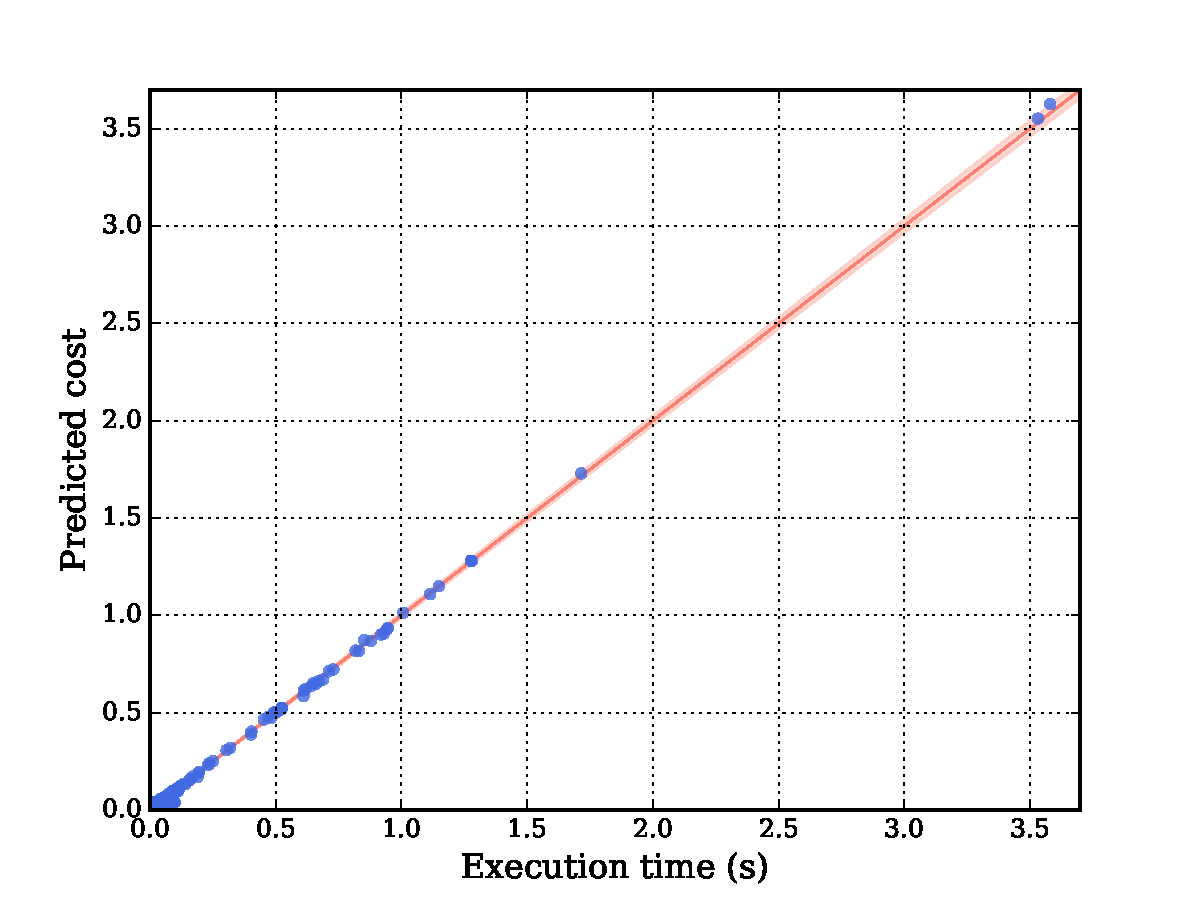
\includegraphics[width=0.9\linewidth]{figs/cost-model.pdf}
    \caption{Linear model fitted from empirical data. The mean absolute error (MAE) for the fitted curve is seven milliseconds.}
    \label{fig:cost-model}
\end{figure}

Figure~\ref{fig:cost-model} compare the work metric with the corresponding execution time for some instances of the test benchmarks.
Notice how the fitted model has a higher relative error for the instances with very short execution time, namely those that run for less than one tenth of a second.
The mean absolute error (MAE) for the fitted curve is seven milliseconds.

\subsection{Comparison with Instructions Per Cycle} \label{sec:ipc-vs-work-metric}

The IPC metric has been widely used for studying performance benefits of hardware optimisations.
Although previous work has suggested the use of IPC for guiding {\itercomp}, in this section we argue in favour of the WP metric over IPC.

The IPC metric differs from the proposed WP metric in a key aspect:
the IPC metric is computed solely based on the final optimised program.
When executing different optimised versions of a program with the same input, both the number of instructions and the number of clock cycles can change.
For this reason, higher IPC does not necessarily translate to shorter execution time (or even fewer clock cycles).

We can illustrate this fact with a very small example as shown in Table~\ref{tab:ipc-example}.
This example shows two versions of a program, namely P1 and P2, and their respective measurements related to IPC.
Although version P1 has twice the IPC of P2, P1 is one cycle slower than P2.
As this example illustrates, the IPC metric can be misleading when compared different versions of the same program.
This problem is only intensified when both the optimisation sequence and the input changes.
In Chapter~\ref{chap:eval} we show empirical evidence for this argument.

\begin{table}[h]
\centering
\begin{tabular}{|c|c|c|c|}
\hline
                       & P1 & P2  \\
\hline
Number of Instructions & 5  & 2   \\
Number of Cycles       & 5  & 4   \\
IPC                    & 1  & 0.5 \\
\hline
\end{tabular}
\caption{Example that illustrates that a higher IPC does not necessarily translate to shorter execution time.}
\label{tab:ipc-example}
\end{table}

On the other hand, WP computes the amount of work based on the unoptimised version of the program, which means that it always measures the same amount of work for the same input, regardless of the optimisations applied on the program.
This is a key aspect that enables the use of the WP metric for guiding {\itercomp}, because a higher WP, which represents work per unit time, naturally translate to shorter execution time.
Moreover, previous work has also presented other arguments against the use of IPC in similar use-case scenarios, as discussed in Chapter~\ref{chap:related}.
  
\section{Online {\IterComp} Infrastructure} \label{sec:oic-infra}

Although {\itercomp} had been originally proposed as an \textit{offline} optimisation strategy, it can also be adapted to work in online scenarios.
Instead of selecting the best optimisation sequence as part of the development time (pre-shipping) of a program, a first version of the program is shipped together with an {\itercomp} mechanism.
In the online scenario, the program is shipped with an initial optimisation sequence and different optimisation sequences are evaluated as the end-user executes the program.
This optimisation strategy is also known as idle-time optimisation, as the re-compilation happens between runs of the program.

LLVM is particularly suitable for iterative compilation as it makes possible to cache a pre-compiled, but still unoptimised, version of the input program in the bitcode format of the LLVM IR.  
This caching allows to speedup the time required for re-compilation as it is able to bypass the frontend phase.
If re-compilation time is critical, it would also be possible to keep only the hot portion of the code in the LLVM bitcode format, while the remaining portion of the code is already compiled to the final object code.
However, this is out of the scope of this thesis and we always re-compile the whole program.

\begin{figure}[htb]
    \centering
    \includegraphics[width=\linewidth]{figs/infra-diagram}
    \caption{Overview of the execution engine for applying {\itercomp}.}
    \label{fig:infra-diagram}
\end{figure}
%\textbf{Describe the process step by step.}

Figure~\ref{fig:infra-diagram} shows an overview of the infrastructure required for applying online {\itercomp}
using WP as the metric of choice for evaluating optimisation sequences.
The online {\itercomp} follows as described bellow:
\begin{enumerate}
\item The program is pre-compiled to the LLVM bitcode format without optimisation.
\item The unoptimised program is instrumented for work profiling.
\item Execution-based optimisation search:
 \begin{enumerate}
   \item The current optimisation sequence is used for the re-compilation of the program.
   \item The program is executed with any input provided by the end-user.
         During the execution of the program, wall-clock time and the work metric are recorded by profiling instrumentation.
   \item If the recorded profiling for the current optimisation can be used to compute an average performance measurement within a small confidence interval,
         then a new optimisation sequence is generated.
         Otherwise, the same optimisation sequence is used for the next execution.
 \end{enumerate}
\end{enumerate}

In this work, we focus mainly on the highlighted components.
The \textit{Work Instrumentation} phase focuses on providing a low-overhead instrumentation for profiling the work metric.
The instrumentation consists of adding a global counter to the program which is used to accumulate the amount of work computed during the program's execution, using the cost model of the instruction set.
A detailed description of the work instrumentation is presented in Section~\ref{chap:instr}.

Notice how the \textit{Work Instrumentation} phase is executed before performing any optimisation to the program.
It is critical so that the work profiling always measure the same amount of work for a given input, regardless of the optimisation sequence applied to the program.
Because the instrumentation is performed before optimising the program, it means that the work profiling derives the linear expression defined in Equation~\ref{eq:linear-work-expression}
based on the unoptimised program.
In other words, the basic blocks and the number of occurrences of the instruction in the basic blocks reflect the unoptimised program.
This particular sequence of compilation guarantees that the amount of work must is only input dependent, but consistent between different optimisation sequences.

%In both phases the goal is to improve the performance of the execution phase, but from different perspectives.
%\textit{(i.)} In the compilation phase we focused on providing a low-overhead instrumentation for profiling the work metric. This phase is responsible to improve performance by lowering the overhead of the work profiling.
%\textit{(ii.)} In the evaluation phase we proposed the use of the WP metric in order to enable {\itercomp} in an online scenario.
%This phase is responsible to improve performance by being able to properly assess different optimisations such that the best optimisation can be selected.
%Chapter~\ref{chap:instr} describes our work profiling strategy and Section~\ref{sec:metric} describes the work-based metric.

%\textbf{Talk about the process of keeping the same optimization for a given input-window and how the optimizations as selected based on the evaluation of these "evidences". Perhaps we could suggest using the Theory of Evidences at this point?!}

As the name suggests, the component called \textit{Optimisation Selector} is responsible for selecting which optimisation sequence to use for the next execution of the program.
It can either keep the same optimisation sequence used in the previous execution or start monitoring the performance of a new optimisation sequence.
An optimisation sequence can be kept for multiple executions of the program in order to gather enough measurement to compute an average performance with small statistical deviations, i.e., for which the confidence interval has a small range.
We call by \textit{Input-Window Size} the number of executions performed using the same optimisation sequence.

\subsection{Real Online Scenarios}

In most online scenarios, it is common for periods of peak usage and idle periods.
For example, mobile devices are usually intensely used during the day, with some idle periods usually when the battery is being re-charged~\citep{mpeis16}.
Similarly, many authors have also considered peak and idle (or underutilised) periods in the context of data centres~\citep{armbrust10,chen12b}.

The proposed infrastructure is very well suited for these real online scenarios\footnote{
However, if idle time is almost non-existent, the proposed infrastructure can still be used by re-compiling the program with a different optimisation while multiple runs of the program are being executed.}.
In particular, periods of peak usage could be used to monitor multiple runs of the program using the same optimisation sequence, collecting the work profiling and measuring its execution time,
while periods of idleness or underutilisation could be leveraged to use the profiling statistics for selecting better optimisations and re-compiling the program.


\section{Instrumentation}

In this section we describe how the computation of the work-metric can be performed during runtime by means of instrumenting the code.
In particular, we adapt the optimal algorithm proposed originally for profiling block frequency~\cite{knuth73,ball94}.
Afterwards, we propose a relaxed instrumentation that focus on further reducing the overhead by considering the trade-off between profiling accuracy and instrumentation overhead.

Because we define work as a linear equation on the block frequency counters, it is possible to embed its computation into the execution of the program.
A naive instrumentation would consists basically of having a global counter that starts with the interception value, $\varepsilon$, and each basic block increments its own cost into the global counter.
Although this instrumentation is easily implemented, it inserts a large amount of overhead into the program.
However, it is possible to insert fewer probes by carefully placing the probes in a way that is possible to reconstruct the complete profiling information~\cite{knuth73,ball94}.

Ball and Larus~\cite{ball94} show that a set of edges represents the minimum number of probes for profiling block frequency if and only if the complementary set of edges forms a spanning tree.
The instrumentation optimises the placement of the probes with respect to a weighing that assigns a non-negative value to each edge in the CFG.
The cost of profiling a set of edges is proportional to the sum of the weights of the edges.
These weights can be obtained either by empirical measurements or heuristic estimations.
In order to minimise the profiling cost, the instrumentation computes the maximum spanning tree for avoiding probing in frequently executed edges.
Although this instrumentation algorithm is proved to produce the optimal placement of probes for well-structured CFGs, it may produce sub-optimal placement for some unstructured CFGs.

Once we have the maximum spanning tree, probes are placed on any edge not in the spanning tree. Figure~\ref{fig:cfg-example} shows an example of a CFG with a maximum spanning tree represented by the black edges, while the edges highlighted in red represent the placement of the probes.

\begin{figure}[htb]
\centering {
  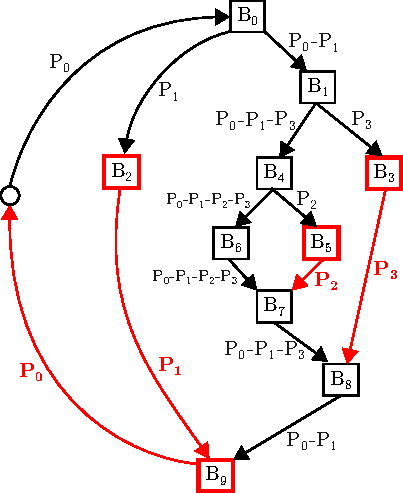
\includegraphics[scale=0.9]{figs/cfg-example.pdf}\\\vspace{1ex}
  \resizebox{0.45\textwidth}{!}{
  %\scalebox{0.8}{
     \begin{minipage}{0.5\textwidth}
     Instrumented value for each probe $P_i$:
     \begin{align*}
     w(P_0) &= w(B_0) + w(B_1) + w(B_4) + w(B_6) + w(B_7) + w(B_8) + w(B_9)\\
     w(P_1) &= w(B_2) - w(B_1) - w(B_4) - w(B_6) - w(B_7) - w(B_8)\\
     w(P_2) &= w(B_5) - w(B_6)\\
     w(P_3) &= w(B_3) - w(B_4) - w(B_6) - w(B_7)
     \end{align*}
     \end{minipage}
  }
}
  \caption{Example of a CFG with its minimum spanning tree in black and the
   basic blocks highlighted in red represent the instrumented basic blocks with
   the placement of the probes.}
  \label{fig:cfg-example}
\end{figure}

In contrast to the naive instrumentation where each basic block records only its own amount of work, with the optimal profiling, the instrumented basic blocks need record an aggregated value of work that represents a path in the CFG.
These values are constructed with some instrumented basic blocks speculatively assuming some paths while other probes correct when these assumptions are wrong (see for example $w(P_0)$ and $w(P_1)$ in Figure~\ref{fig:cfg-example}).

\begin{lstlisting}[caption={Post-processing of the CFG for populating all edge flows based on the collected probes.}, label={lst:populateEdgeFlows}, float]
// Inputs: CFG with the known edges flows from
//         the cotree (collected probes).
// Output: Updated CFG with all edge flows.
populateEdgeFlows(G) {
  changed = true
  while changed:
    changed = false
    for B in G.vertices():
      unIN = count( G.unknownIncomingEdges(B) )
      unOUT = count( G.unknownOutgoingEdges(B) )
      if unIN==0 and unOUT==1:
        //sum known incoming and outgoing edges
        sIN = sum( G.incomingEdges(B) )
        sOUT = sum( G.outgoingEdges(B) )
        //update unknown outgoing edge in B
        //with (sIN-sOUT)
        G.setUnknownOutgoingEdge(B, (sIN-sOUT))
        changed = true
      if unIN==1 and unOUT==0:
        //sum known incoming and outgoing edges
        sIN = sum( G.incomingEdges(B) )
        sOUT = sum( G.outgoingEdges(B) )
        //update unknown incoming edge in B
        //with (sOUT-sIN)
        G.setUnknownIncomingEdge(B, (sOUT-sIN))
        changed = true
}
\end{lstlisting}


Because the algorithm for the optimal placement of the probes is proved to uniquely compute the block frequencies by propagating the probe counts, we adapt this algorithm in order to compose the aggregated values that will be instrumented in each probe, based on our model of computational work, $\Delta W$, derived from the basic block frequencies (see Section~\ref{sec:metric}).
We perform a similar propagation of the probes in a symbolic fashion, as illustrated in Figure~\ref{fig:cfg-example}.
This symbolic propagation of the probes is implemented by the data-flow analysis described in Algorithm~\ref{alg:populateEdgeInfo}, and the final aggregated values are extracted from the edge information as described by Algorithm~\ref{alg:instrValue}.

The data-flow analysis in Algorithm~\ref{alg:populateEdgeInfo} keeps two sets for each edge, namely, the increment and the decrement sets.
We consider that both sets represent the \textit{edge expressions} shown in Figure~\ref{fig:cfg-example}, for which we define a \textit{symbolic sum} by computing the union of the increment and decrement sets, respectively, with the appropriate cancellation of common elements.
This data-flow analysis is based on the invariant that the symbolic sum of all the incoming edges must equals the symbolic sum of the outgoing edges.
For example, the symbolic sum of the incoming edges of the basic block $B_8$ is $P_0 - P_1$, where $P_3$ is cancelled out.

%By construction, the \textit{symbolic experssions} of a basic block, i.e., the \textit{symbolic sum} of the incoming edges (or outgoing edges) of a basic block, has the following properties:
%\begin{enumerate}
%\item Probes in the increment set either (post-)dominates or is (post-)dominated by the given basic block;
%\item Probes in the decrement set are (post-)dominated by the probes in the increment set;
%\item Probes in the decrement set and the given basic block are in exclusive paths from the virtual node of the CFG to the (post-)dominators in the increment set;
%\end{enumerate}
%From property (1) it follows that whenever the given basic block is executed, exactly one of the probes in the increment set is executed.
%From properties (2) and (3), it follows that whenever a probe in the decrement set is executed, although the given basic block is not executed, one of the probes in the decrement set is executed.

Algorithm~\ref{alg:instrValue} reads the edge information for each basic block by computing the symbolic sum of their respective incoming edges (or outgoing edges).
From these \textit{edge expressions}, we are able to compose the aggregated value of the probes.
The positive terms in the edge expression of a basic block indicate that the amount of work of this basic block will be incremented in the probes represented by these positive terms, similarly, the negative terms indicate that the amount of work of this basic block will be decremented in the probes represented by these negative terms.
For example, because the edge expression for the basic block $B_8$ is $P_0 - P_1$, the amount of work of $B_8$, denoted by $w(B_8)$, is incremented in probe $P_0$ and decremented in $P_1$.

\begin{lstlisting}[caption={Pseudocode that describes how the edge information is used in order to extract the value that will be computed in a given instrumented basic block $B_I$. This algorithm could equally be implemented based on the predecessors.}, label={lst:instrValue}, float]
// Inputs: 1) CFG with the known edges flows
//            of the chords.
//         2) Basic block targeted for probing.
// Output: Work value to be incremented by the
//         given probe B.
instrValue(G, B, inc, dec) {
  value = 0
  for B in G.vertices():
    incB = set()
    decB = set()
    for succB in G.successor(B):
      incB = incB union inc[G.getEdge(B, succB)]
      decB = decB union dec[G.getEdge(B, succB)]
    if B in (incB - decB):
      value = value + w(B)
    if B in (decB - incB):
      value = value - w(B)
  return value
}
\end{lstlisting}


\subsection{Relaxed Instrumentation}

Although the optimal instrumentation significantly reduces the profiling overhead when compared to the naive instrumentation, from an average overhead of 79\% to 13\%, in some critical cases, even the optimal instrumentation can have an overhead of about 70\% (see benchmark \texttt{adpcm\_d} in Figure~\ref{fig:overhead-O3}).
In order to further reduce the overhead in these critical cases, we propose a relaxed instrumentation by trading off accuracy and overhead.
While the optimal placement of probes tries to place probes in edges that are less likely to be executed, the relaxation focus on removing probes that are more likely to be executed but add little to the work metric.

\begin{figure}[h]
  \centering
  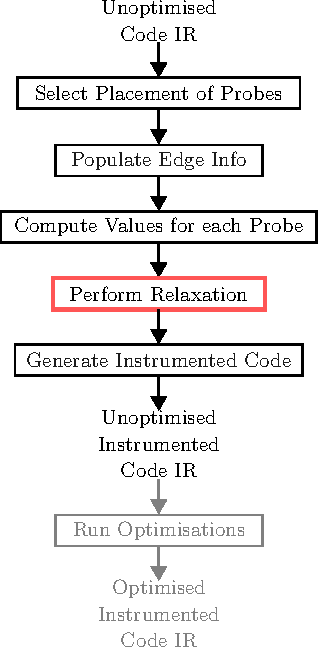
\includegraphics[scale=0.9]{figs/relax-instr-diagram.pdf}
  \caption{Overview of the work instrumentation algorithm, including the relaxation technique.}
  \label{fig:relax-instr-diagram}
\end{figure}

%\begin{figure*}[htb]
%    \centering
%    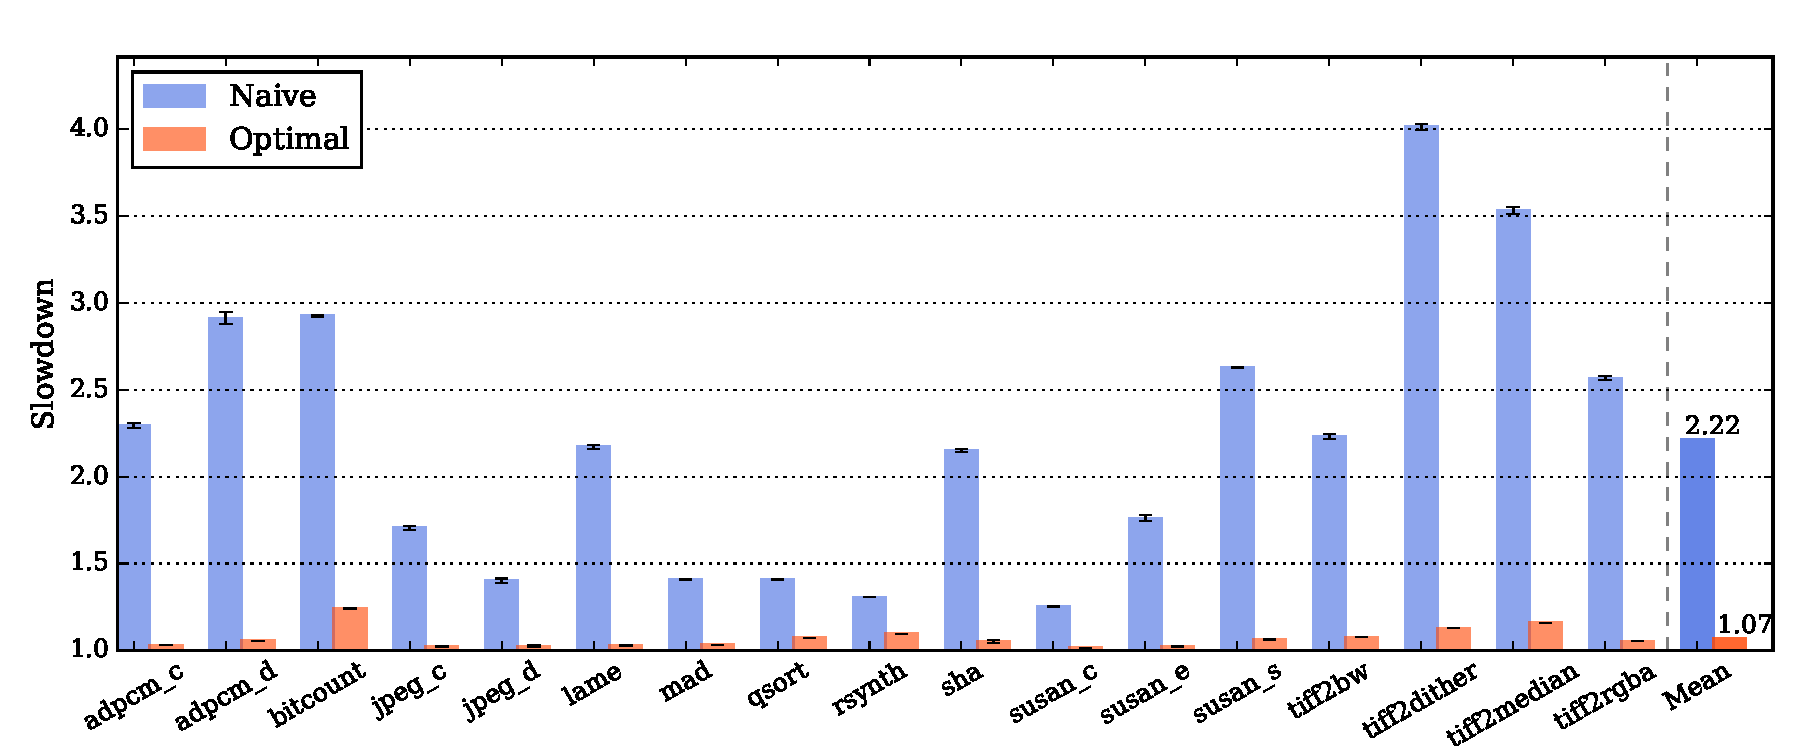
\includegraphics[width=\textwidth]{figs/overhead-O0.pdf}
%    \caption{Comparison between the naive and optimal instrumentation
%              with no compiler optimisation.}
%    \label{fig:overhead-O0}
%\end{figure*}

%Define an DAG of a CFG as a directed graph which may contain cycles if they have known constant trip counts.
Figure~\ref{fig:relax-instr-diagram} shows an overview of the relaxed instrumentation algorithm.
The highlighted step is introduced by the relaxed instrumentation on top of the previously defined optimal profiling.
The relaxed instrumentation performs a post-processing on the resulting instrumentation of the optimal algorithm.
This post-processing identifies probes that add little to the work metric, and removes their instrumentation.
In order to guarantee an upper bound for the dynamic error in the profiling measurement, the relaxation algorithm applies a constrained post-processing on a per DAG (directed acyclic graph) basis.
By constraining the relaxation within each DAG by a maximum allowed static error, it guarantees that the overall relaxation will also be constrained by the same bound.


The relaxation starts by extracting DAGs (directed acyclic graphs) from the CFG, as illustrated in Figure~\ref{fig:cfg-relax-example}.
First, the algorithm extracts all the subgraphs that represent a loop or the outer most region of the function.
Section~\ref{sec:natural-loops} explains how loops can be identified in the CFG.
Afterwards, these subgraphs are transformed into DAGs by ignoring the backedge and also by considering that any loop within the subgraph is never executed, i.e., only the headers of the inner loops are actually included into the DAG.
Figure~\ref{fig:cfg-relax-example} shows a CFG partitioned into two DAGs (consider only basic blocks and edges completely inside the yellow and green boundaries).
%
%LLVM has a Scalar Evolution Analysis which is used primarily to analyse expressions involving induction variables in loops~\cite{pop05}.
%An induction variable is a variable that is increased or decreased by a fixed amount on every iteration of a loop or is a linear function of another induction variable.
%
%This Scalar Evolution Analysis provides a way to compute \textit{small} constant trip counts (where \textit{small} is defined by a threshold).

\begin{figure}[h]
  \centering
  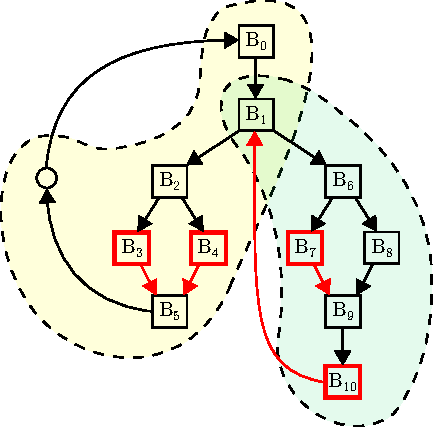
\includegraphics[scale=1]{figs/cfg-relax-example.pdf}
  \caption{Example of a CFG containing a loop and its decomposition into DAGs when applying the relaxation.
           The DAGs are the subgraphs within the dashed boundaries.}
  \label{fig:cfg-relax-example}
\end{figure}

\newpage
\begin{lstlisting}[caption={Optimal placement of probes for block frequency.}, label={lst:instrumentCFG}]
// Input: CFG	
relaxInstrumentation(G) {
  for loop in G:
     DAG = colapseInnerLoops(loop)
     relaxInstrumentedDAG(DAG)
  DAG = colapseInnerLoops(G)
  relaxInstrumentedDAG(DAG)
}
\end{lstlisting}

For every DAG with a set of probes $\{P_0, P_1, \ldots, P_k\}$, we relax the profiling accuracy by selecting a subset of the probes to be removed, subject to the maximum allowed percentage error, $M$.

We model the relaxation as a 0-1 Knapsack problem:
\begin{equation*}
\begin{aligned}
& \textrm{maximise }\quad \sum_{i=0}^{k} f(P_i)x_i \\
& \textrm{subject to }\quad \sum_{i=0}^{k} \varepsilon(P_i)x_i \leq M
\end{aligned}
\end{equation*}
\[
x_i\in\{0,1\}, i\in\{0,\ldots,k\}
\]
where $f(P_i)$ is the execution frequency of probe $P_i$, $x_i$ denotes the probes selected for removal, and $\varepsilon(P_i)$ is the percentage error of removing probe $P_i$ relative to the minimum work value possible to compute in the DAG, i.e., if $m$ is the minimum amount of work possible to be computed when executing the DAG, then $\varepsilon(P_i) = \frac{\omega(P_i)}{m}$.
Because the percentage error is computed based on the path with the minimum amount of work, $\varepsilon(P_i)$ represents the maximum error possible that would be incurred when removing probe $P_i$.
Furthermore, by constraining the percentage error of every DAG below a given threshold, we guarantee that the final error of the relaxation will always be bounded by the threshold, as demonstrated by Proposition~\ref{prop:relax-bound}.

\begin{prop}\label{prop:relax-bound}
Let $n_i$ be the number of times a given DAG $i$ is executed, $r_i$ be the total relaxation (amount of work removed) in DAG $i$, and $m_i$ be its minimum amount of work.
If $\frac{r_i}{m_i} \leq M$ for every $i$,
then the final error of the relaxation will always be bounded by the same threshold.
\end{prop}
\begin{proof}
We can model the overall error of the relaxation as:
\[
1 - \frac{n_1(m_1 - r_1) + n_2(m_2 - r_2) + \ldots + n_k(m_k - r_k) + c}{n_1m_1 + n_2m_2 + \ldots + n_km_k + c}
\]
That is,
%\begin{equation*}
\begin{gather*}
 1 - \frac{n_1m_1 + n_2m_2 + \ldots + n_km_k + c}{n_1m_1 + n_2m_2 + \ldots + n_km_k + c} + \frac{n_1r_1 + n_2r_2 + \ldots + n_kr_k}{n_1m_1 + n_2m_2 + \ldots + n_km_k + c} = \\
 \frac{n_1r_1 + n_2r_2 + \ldots + n_kr_k}{n_1m_1 + n_2m_2 + \ldots + n_km_k + c}
\end{gather*}
%\end{equation*}
If $\frac{r_j}{m_j}$ is the maximum ratio $\frac{r_i}{m_i}$ for every $i$, then
\begin{equation*}
\begin{aligned}
 \frac{n_1r_1 + n_2r_2 + \ldots + n_kr_k}{n_1m_1 + n_2m_2 + \ldots + n_km_k + c} &\leq\\
 \frac{n_1r_j + n_2r_j + \ldots + n_kr_j}{n_1m_j + n_2m_j + \ldots + n_km_j + c} &\leq\\
 \frac{n_1r_j + n_2r_j + \ldots + n_kr_j}{n_1m_j + n_2m_j + \ldots + n_km_j} & 
\end{aligned}
\end{equation*}
If $N = max\{n_i$ for every $i\}$, then
\begin{equation*}
\begin{aligned}
 \frac{n_1r_j + n_2r_j + \ldots + n_kr_j}{n_1m_j + n_2m_j + \ldots + n_km_j} &\leq\\
 \frac{Nr_j + Nr_j + \ldots + Nr_j}{Nm_j + Nm_j + \ldots + Nm_j} &=\\
 \frac{Nkr_j}{Nkm_j} = \frac{r_j}{m_j} &\leq M
\end{aligned}
\end{equation*}
\end{proof}


\begin{lstlisting}[caption={Optimal placement of probes for block frequency.}, label={lst:instrumentCFG}]
// Input: CFG	
relaxInstrumentedDAG(DAG){
   P = ProbesIn(DAG)
   m = minWork(DAG,P)
   K = createKnapsackModel(P,m)
   Bag = solveKnapsack(K)
   for B in (P-Bag):
     removeProbe(B)
}
\end{lstlisting}

The necessary block-frequency information for optimising both the placement of probes can be acquired from profiles of previous executions of the program or by a static heuristic of the CFG during compilation.

For our experiments, we implemented two solvers for the 0-1 Knapsack problem:
the optimal brute-force solver;
the greedy heuristic based on sorting the items~\citep{dantzig57}.
We use the brute-force solver for DAGs with a small number of probes and the greedy heuristic when the number of probes is greater than a threshold.
Some of the benchmarks have DAGs with several hundreds of probes, which could result in a long compilation time.

\subsection{Whole Program Relaxation}

In some cases, the proposed relaxation can be very conservative, because it considers the static error of removing probe $P_i$ relative to the minimum work possible of a DAG, in order to be able to guarantee that the dynamic error will be bounded by a given threshold.
This conservatism can be overly restrictive in some cases, resulting in a negligible overhead reduction but also causing just a negligible dynamic error to the work profiling.

In some cases, this overly restrictive conservatism may be unnecessary.
For these cases, we propose an adapted version of the relaxation algorithm that operates on the whole program.
Traditionally, compilers optimisations are performed on the function-level, or at best on a per module basis.
Whole program optimisation (WPO) means that the compiler considers all compilation units of the program and optimises them using the combined knowledge of how they are used together.

The whole program relaxation works by using block-frequency profiling from previous executions.
By having this profiling information, the \textit{whole program relaxation} is able to compute the error of removing a given probe in terms of the whole program's execution,
and then use this error values for selecting a subset of all the probes to be removed.

For a program with a set of probes $\{P_0, P_1, \ldots, P_k\}$, we model the whole program the relaxation as the following 0-1 Knapsack problem:
\begin{equation*}
\begin{aligned}
& \textrm{maximise }\quad \sum_{i=0}^{k} f(P_i)x_i \\
& \textrm{subject to }\quad \sum_{i=0}^{k} \varepsilon(P_i)x_i \leq M
\end{aligned}
\end{equation*}
\[
x_i\in\{0,1\}, i\in\{0,\ldots,k\}
\]
where $f(P_i)$ is the execution frequency of the instrumented basic block $P_i$, $x_i$ denotes the probes selected for removal, $M$ is the error threshold, and $\varepsilon(P_i)$ is the percentage error of removing probe $P_i$ relative to the profiled global work, i.e.,
if $\Delta W$ is the work value for the whole program's execution, computed from the basic block frequencies profiled from previous executions, the error for a given probe $P_i$ is
\[
\varepsilon(P_i) = \frac{\omega(P_i)f(P_i)}{\Delta W}.
\]

Contrary to the per DAG relaxation, the whole program relaxation is not guaranteed to be bounded by the error threshold $M$,
as it depends on the representativity % representativeness
 of the profiling information provided to the whole program relaxation.
 

\section{Experimental Evaluation}

In this section we discuss our experimental evaluation.
First we describe the benchmarks with datasets used in the experiments.
Afterwards, we discuss our results concerning the instrumentations for profiling our work metric.
Finally we present the results of the online {\itercomp}.

We implemented the instrumentations in LLVM 4.0.
The target platform is a Linux-4.4.27 system with an Intel Core i7-4770 3.40GHz Skylake~CPU with 16~GiB RAM.

\subsection{Benchmarks}

For the experimental evaluation we have used a subset of the \textit{KDataSets} benchmark suit, which is the same benchmark and dataset suit used by Chen~\etal~\cite{chen10,chen12a}.
The KDataSets contains 1000 different inputs for each one of its benchmark programs.
These benchmarks cover a broad spectrum of application scenarios, ranging from simple embedded signal-processing tasks to common mobile-phone and desktop tasks.
The different inputs try to capture distinct characteristics in terms of workload sizes and how these workloads exercise different control flow paths.
A summary of the benchmarks and dataset suit is shown in Table~\ref{tab:kdatasets}.

\begin{table}[h]
\centering
\scalebox{.8}{
\begin{tabular}{|c|c|c|c|}
\hline
\textbf{Program} & \textbf{LOC}    & \textbf{Input file size}            & \textbf{Input description}              \\ \hline % Domain
qsort         & 154    & 32K-1.8M                   & 3D coordinates                 \\ \hline
jpeg\_d       & 13501  & 3.6K-1.5M                  & JPEG images                    \\ \hline
jpeg\_c       & 14014  & 16K-137M                   & PPM images                     \\ \hline
tiff2bw       & 15477  & \multirow{4}{*}{9K-137M}   & \multirow{4}{*}{TIFF images}   \\ \cline{1-2}
tiff2rgba     & 15424  &                            &                                \\ \cline{1-2}
tiffdither    & 15399  &                            &                                \\ \cline{1-2}
tiffmedian    & 15870  &                            &                                \\ \hline
susan\_c      & 1376   & \multirow{3}{*}{12K-46M}   & \multirow{3}{*}{PGM images}    \\ \cline{1-2}
susan\_e      & 1376   &                            &                                \\ \cline{1-2}
susan\_s      & 1376   &                            &                                \\ \hline
adpcm\_c      & 210    & 167K-36M                   & WAVE audios                    \\ \hline
adpcm\_d      & 211    & 21K-8.8M                   & ADPCM audios                   \\ \hline
lame          & 14491  & 167K-36M                   & WAVE audios                    \\ \hline
rsynth        & 4111   & 0.1K-42M                   &  Text files                    \\ \hline
sha           & 197    & 0.6K-35M                   & Files of any format            \\ \hline
\rowcolor{gray!20}
bitcount      & 460    &  -                         & Numbers: random                \\ \hline
\rowcolor{gray!20}
dijkstra      & 163    & 0.06K-4.3M                 & Adjacency matrices             \\ \hline
\rowcolor{gray!20}
patricia      & 290    & 0.6K-1.9M                  & IP and mask pairs              \\ \hline
\rowcolor{gray!20}
mad           & 2358   & 28K-27M                    & MP3 audios                     \\ \hline
\rowcolor{gray!20}
%gsm           & 3806   & 83K-18M                    & Sun/NeXT audios                \\ \hline
ghostscript   & 99869  & 11K-43M                    & Postscript files               \\ \hline
\rowcolor{gray!20}
%ispell        & 6522   & \multirow{3}{*}{0.1K-42M}  & \multirow{3}{*}{Text files}    \\ \cline{1-2}
%rsynth        & 4111   &                            &                                \\ \cline{1-2}
stringsearch  & 338    &  0.1K-42M                 &  Text files                     \\ \hline
\rowcolor{gray!20}
%blowfish\_e   & 863    & 0.6K-35M                   & Files of any format            \\ \hline
%blowfish\_d   & 863    & 0.6K-35M                   & Encrypted files                \\ \hline
%pgp\_e        & 19575  & 0.6K-35M                   & Files of any format            \\ \hline
%pgp\_d        & 19575  & 0.4K-18M                   & Encrypted files                \\ \hline
%rijndael\_e   & 952    & 0.6K-35M                   & Files of any format            \\ \hline
%rijndael\_d   & 952    & 0.7K-35M                   & Encrypted files                \\ \hline
CRC32         & 130    & 0.6K-35M                   & Files of any format            \\ \hline
\rowcolor{gray!20}
bzip2e        & 5125   & 0.7K-57M                   & Files of any format            \\ \hline
\rowcolor{gray!20}
bzip2d        & 5125   & 0.2K-25M                   & Compressed files               \\ \hline
\end{tabular}
}
\caption{Description of the KDataSets with 1000 inputs for each benchmark (Chen~\etal~\cite{chen10,chen12a}).}
\label{tab:kdatasets}
\end{table}

The shaded (grey) benchmarks in Table~\ref{tab:kdatasets} represent the benchmarks used for training the cost model used for computing the weight of the instructions for the work metric.
These same training benchmarks were also used for collecting a fixed set of optimisations for the {\itercomp}.
The remaining (white) benchmarks are used for the experimental evaluation.

\subsection{Evaluation of the Instrumentation}

\begin{figure*}[htp]
    \centering
    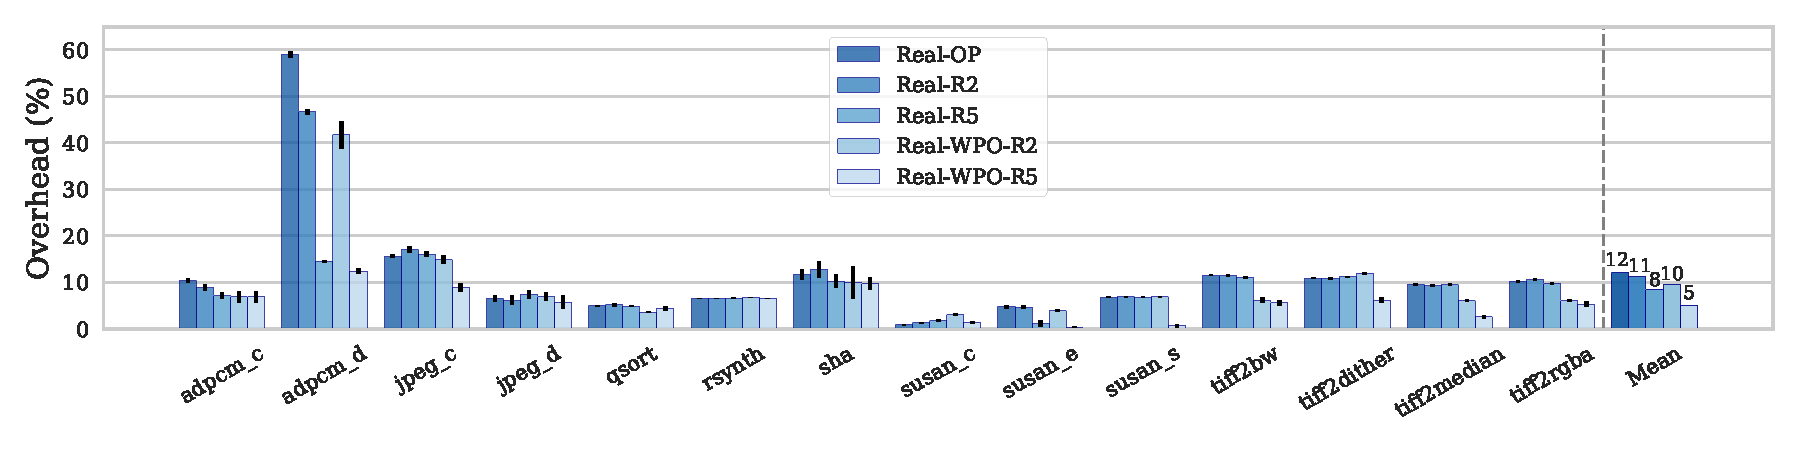
\includegraphics[width=\textwidth]{figs/overhead-O3.pdf}
    \caption{Overhead of the instrumentations compiled with {\texttt{-O3}}.}
    \label{fig:overhead-O3}
\end{figure*}

Figure~\ref{fig:instr} shows percentage of instrumented basic blocks for the optimal and the relaxed instrumentation with different relaxation thresholds.
The naive instrumentation always has 100\% of the basic blocks instrumented, by definition.

\begin{figure*}[htp]
    \centering
    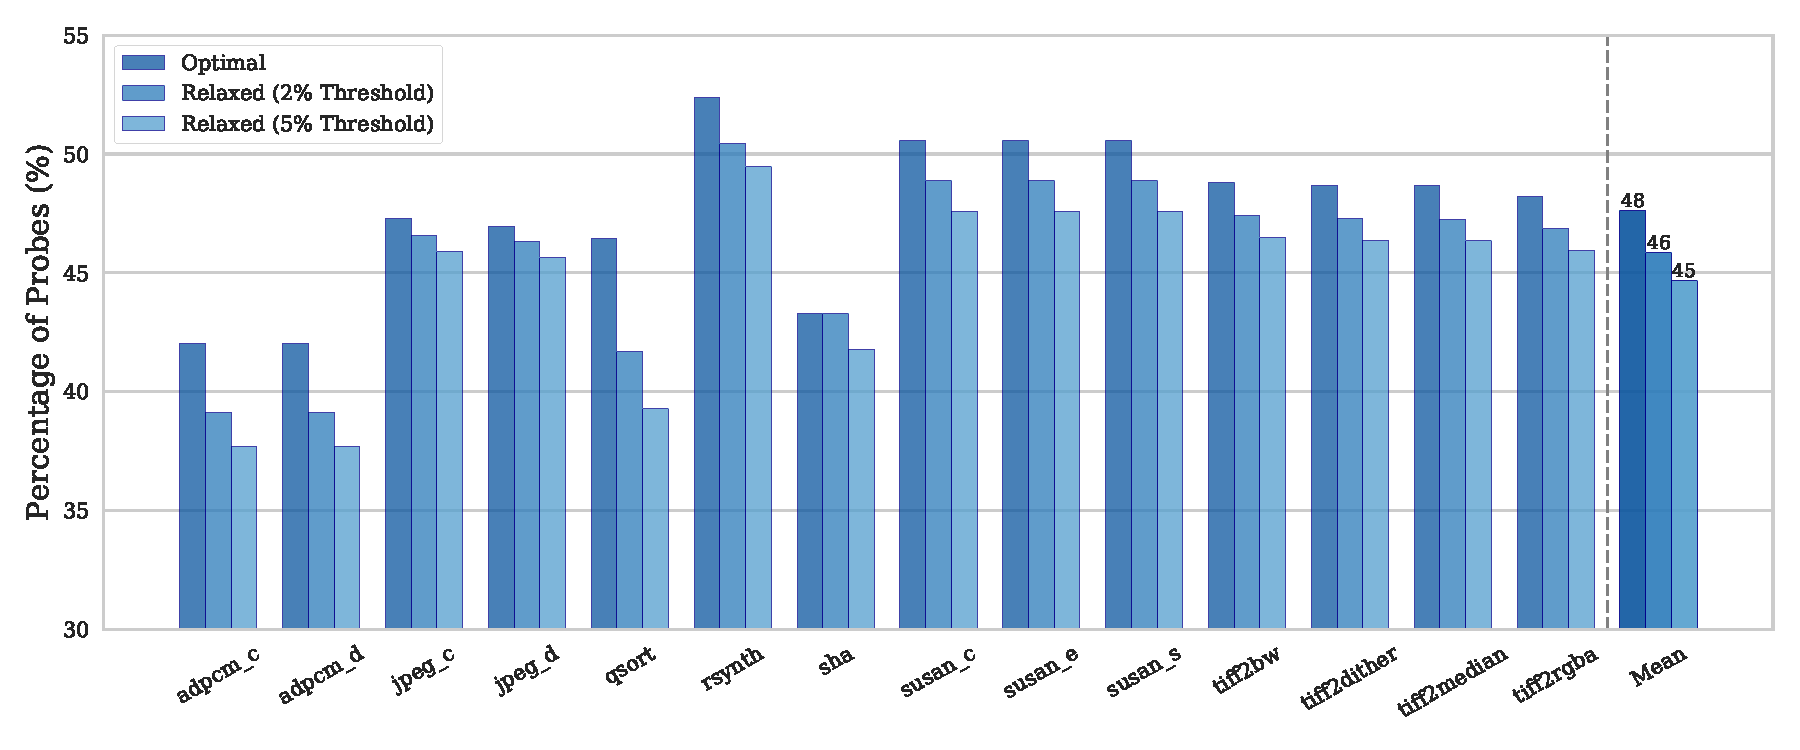
\includegraphics[width=\textwidth]{figs/num-probes.pdf}
    \caption{Percentage of instrumented basic blocks for the optimal and the relaxed instrumentation with different relaxation thresholds.}
    \label{fig:num-probes}
\end{figure*}

The \texttt{adpcm\_d} benchmark is the most critical case amongst the used benchmarks, with a overhead of about 66\% with the optimal instrumentation.
This benchmark consists mainly of a single hot loop with several branches inside it.
The relaxation algorithm is able to reduce this overhead down to about 52\% (with an error threshold of 1\%) and 19\% (with an error threshold of 2\%) by removing only one and two probes from the hot loop, respectively.
These two removed probes were placed in branches, inside the hot loop, with a high probability of being taken, but with a small contribution to the work measured in the loop.

%In this section we discuss the three baseline implementations that will be used for assessing the quality of the proposed metric.

%\vspace{1ex}
%\noindent \textbf{{\Itercomp} over a single input}

%Most of the existing {\itercomp} studies find the best optimisation though repeated runs on the same input.
%Although this approach will usually lead to sub-optimal performance across large input datasets, it provides a good baseline when considering the complexity and resonably low compile-time regarding iterative optimising compilers.
%If $M$ is the total number of combinations of compiler optimisations, this approach requires $O(M)$ runs of the program being optimised.
%We can consider two main scenarios:
%\textit{($i$ - best case scenario)} after selecting the optimisation over each individual input, consider the one with best performance across the whole input dataset;
%\textit{($ii$ - expected scenario)} after selecting the optimisation over each individual input, consider the average case of their performance across the whole input dataset.

%\vspace{1ex}
%\noindent \textbf{{\Itercomp} across large input datasets}

%Recent work on {\itercomp} have been targeting optimisation across multiple inputs~\cite{fursin07,chen10,chen12a}.
%If $N$ is the number of input test cases and $M$ is the total number of combinations of compiler optimisations, they perform a total of $O(NM)$ runs of the program being optimised.
%Similarly to what have been discussed previously, there are different ways for how to determine the optimal combination of compiler optimisations across multiple inputs.
%It is possible to tune the selection of the program-optimal combination to minimise risk or to maximise average performance.
%A compromise-based selection criterion could be to maximise average speedup with minimised variance.

%\vspace{1ex}
%\noindent \textbf{{\Itercomp} based on the IPC metric}

%While the previous two baselines addresses two opposite aspects of {\itercomp}, namely, compile-time efficiency and performance of the generated code, we also intend to compare against IPC as the competing baseline.
%The main reason for comparing against IPC is because it has been proposed as a metric for comparing the performance of two optimisations running on two distinct inputs.
%If $M$ is the total number of combinations of compiler optimisations, this approach requires $O(M)$ runs of the program being optimised.

\subsection{Evaluation of the Online {\IterComp}}

For comparison, we use four configurations\footnote{A configuration using the WPO relaxation was not used due to the time necessary for executing the experiments.}.
In all configurations, the same optimisation sequence is used for multiple inputs, using a dynamic input-window size, as explained in Section~\ref{sec:oic-infra}.
The average performance over the input window provides an estimate for the overall performance of the optimisation sequence across distinct inputs.
The optimisation sequences are ranked based on their average performance, and the best optimisation sequence is selected.
%When selecting the best optimisation sequence, they are ranked by the average of their performance measurement, using the WP metric, except for the Oracle-RM which uses the real speedup over \texttt{-O0}.
\begin{itemize}
\item \textbf{Oracle-RM} executes the program multiple times for each input, measuring the real speedup for each optimisation sequence, and then uses the real speedup over {\flagstype -O0} for comparing the optimisation sequences.
  The speedups are computed based on the wall-clock time.
  In order to reduce noise, the program is executed several times for the same input, until the confidence interval was no larger than 1\% for a 99\% confidence.
\newpage
\item \textbf{Oracle-PP} represents an oracle with a \textit{perfect} non-intrusive profiling.
  Although it uses the WP metric for comparing optimisation sequences, this oracle also avoids noise in its measurements by also executing the program multiple times for each input.
  The first execution is used for profiling the work metric.
  The remaining executions are used for measuring the wall-clock time without using the work profiling.
\item \textbf{Real-OP} corresponds to the online {\itercomp} as it would be applied in a real online scenario.
  For each optimisation, a random sample of inputs is selected, and the program is executed only once with each input.
  When executing each input, it uses the optimal work instrumentation for profiling the work metric.
  The average of the WP for the sample of inputs is then used for selecting the best optimisation.
\item \textbf{Real-R5} is similar to the {Real-OP}.
  It also corresponds to the online {\itercomp} as it would be applied in a real online scenario.
  For each optimisation, a random sample of inputs is selected, and the program is executed only once with each input.
  When executing each input, it uses the relaxed work instrumentation, with a 5\% threshold, for profiling the work metric.
  The average of the WP for the sample of inputs is then used for selecting the best optimisation.
\item \textbf{Real-IPC} corresponds to the online {\itercomp} based on the IPC metric.
  For each optimisation, a random sample of inputs is selected, and the program is executed only once with each input.
  The average of the IPC metric for the sample of inputs is then used for selecting the best optimisation.
\end{itemize}
The comparison between Oracle-RM and Oracle-PP is useful for validating the use of the WP metric for guiding {\itercomp}, while the other configurations demonstrate the viability of applying the online {\itercomp} in a real scenario.

Figure~\ref{fig:window-size} shows the average input-window size for each benchmark and configuration.
It shows that we can have a statistically sound measurement of the performance metric using just a small number of inputs.

\begin{figure*}[htb]
    \centering
    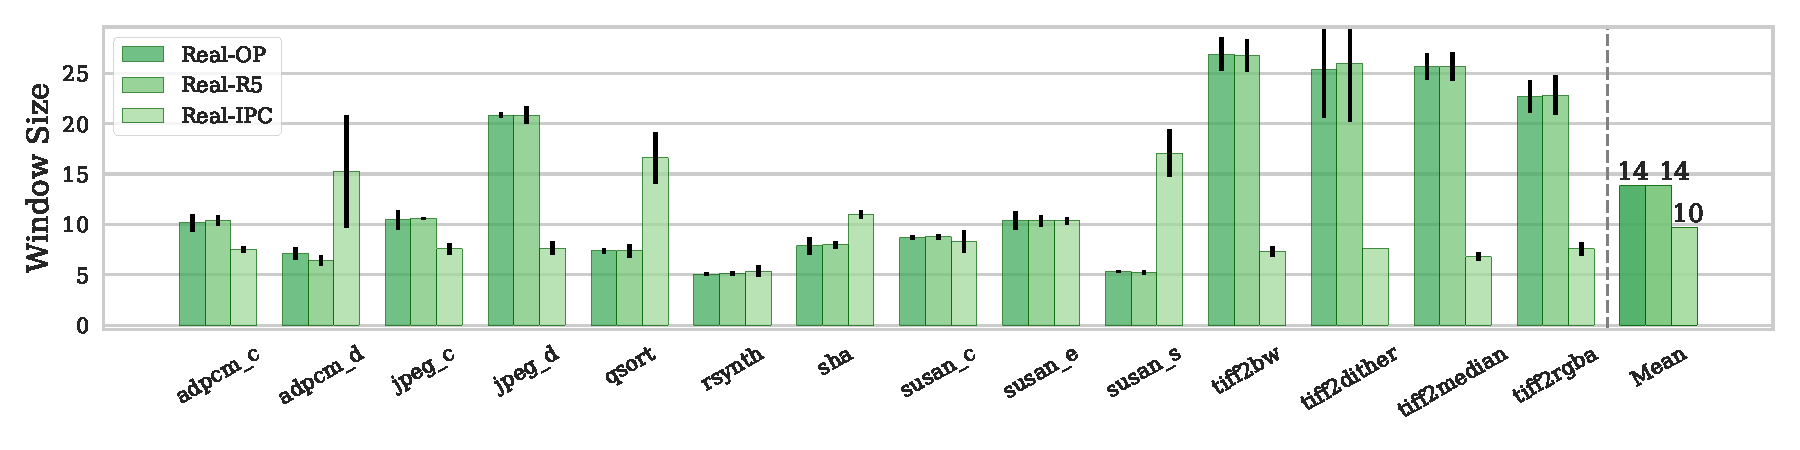
\includegraphics[width=\textwidth]{figs/window-size.pdf}
    \caption{Average input-window sizes observed during the online {\itercomp}.}
    \label{fig:window-size}
\end{figure*}

\subsection{The Set of Optimisation Sequences}

For the purpose of evaluating the use of the WP metric with {\itercomp}, we collected in advance a fixed set of optimisation sequences.
The reason for using this fixed set, as explained in Section~\ref{sec:oic-infra}, is because this thesis is focused on other components of the infrastructure for performing {\itercomp} and we assume that a good generator of optimisation sequences will be used in a real online scenario.
This set contains 500 optimisation sequences collected in a random search using the training benchmarks.
These optimisation sequences contain an average of 40 individual optimisation passes, including repetitions, with a maximum of 119 optimisation passes, but it also contains optimisation sequences which consist of a single flag, such as the default optimisations {\flagstype -O1}, {\flagstype -O2}, {\flagstype -O3}, {\flagstype -Os}, and {\flagstype -Oz}.

  \begin{minipage}{0.9\textwidth}
     \vspace{1em}
     \noindent\textbf{Example of a short optimisation sequence:}\vspace{-1ex}
     \justify{\flagstype -mem2reg -simplifycfg -constprop -dce}
  \end{minipage}

  \begin{minipage}{0.9\textwidth}
     \vspace{1em}
     \noindent\textbf{Example of a long optimisation sequence:}\vspace{-1ex}
     \justify{\flagstype -globalopt -reassociate -instcombine -loop-rotate -block-freq -deadargelim -early-cse -sroa -argpromotion -sccp -tbaa -barrier -constmerge \mbox{-loop-vectorize} -domtree -basicaa -memdep -basiccg -memcpyopt \mbox{-constprop} -adce -globaldce -mem2reg -constmerge \mbox{-globaldce} -constprop -instsimplify -dse -dce -simplifycfg -loop-unroll -reassociate -constprop \mbox{-globaldce} -instsimplify -adce -constmerge -bb-vectorize -dce -mergefunc -simplifycfg -dse -loop-unroll -globaldce}
  \end{minipage}

  \begin{minipage}{0.9\textwidth}
     \vspace{1em}
     \noindent\textbf{Example of an optimisation sequence which includes {-O3}:}\vspace{-1ex}
     \justify{\flagstype -O3 -adce -globaldce -simplifycfg -memcpyopt -reassociate -mergefunc \mbox{-dce} -dse}
     \vspace{2em}
  \end{minipage}

Repeating the same optimisation pass can be beneficial and usually expected by other passes.
For example, the {\flagstype -loop-simplify} pass is used for transforming loops into a canonical form by inserting pre-header and exit basic blocks.
Although this pass inserts jumps due to redundant basic blocks, this canonical form can be favourable to other loop optimisations.
Because of the redundant basic blocks, this optimisation pass expects that the {\flagstype -simplifycfg} will eventually be executor later on the optimisation pipeline.
Another example of such inter-relation between transformations concerns the {\flagstype -licm} and {\flagstype -mem2reg} passes.
The {\flagstype -licm} pass is responsible for moving invariant code out from the loop body.
It usually creates new local variables, using memory access operations, for assisting with the code manipulation, which means that the executing the {\flagstype -mem2reg} pass afterwards would be useful as a cleanup pass for removing the extra memory accesses generated.
However, many of the analysis required for identifying loop invariant also benefit from the transformations performed by the {\flagstype -mem2reg} pass.
These examples illustrate the importance of repeating optimisation passes.
Moreover, they illustrate the intricate relation amongst several transformations.

However, all optimisation sequences in the set of optimisations were generated completely at random, without using any knowledge of individual transformations.
Each optimisation sequence was generated in two steps: \textit{(1)} randomly selects the number of flags; \textit{(2)} randomly selects the flags, allowing repetitions.
Afterwards, this randomly generated optimisation sequence would be included in the set of optimisation sequences only if it was able to improve the performance of a training benchmark, also selected at random, in respect of the {\flagstype -O3} default optimisation.
This process was repeated until we obtained all the 500 distinct optimisation sequences.

\subsection{Performance Evaluation}

In order to evaluate the quality of the final optimisation sequences selected by the {\itercomp} search, we compare their speedup by measuring wall-clock time of the benchmarks when compiled with the standard {\flagstype -O3} optimisation.
For each benchmark, after selecting the final optimisation sequence, we compute the average speedup over all the 1000 input dataset.
When measuring the wall-clock time for each input, to reduce noise, we execute the same input until we have a statistically sound measurement, i.e. we execute until we have an interval no larger than 1\% with 99\% confidence.
Figure~\ref{fig:speedups} shows these average speedups over all the 1000 input dataset.
This figure shows that the best optimisation sequence selected with the Oracle-PP is very close to the performance of the best optimisation sequence selected with the Oracle-RM.
This result is important for demonstrating that a work-based metric has the potential to produce good results in a real online scenario, where there is the restriction that programs execute distinct inputs only once.
Moreover, the evaluation also indicates that the use of relaxation algorithms does not degrade the optimisation search,
it might even benefit the {\itercomp} as it tends to insert smaller interferences in the performance measurement.
Finally, Figure~\ref{fig:speedups} also presents the results of {\itercomp} guided by IPC, which is futher discussed in Figure~\ref{fig:ipc-vs-work}.

\begin{figure*}[htb]
    \centering
    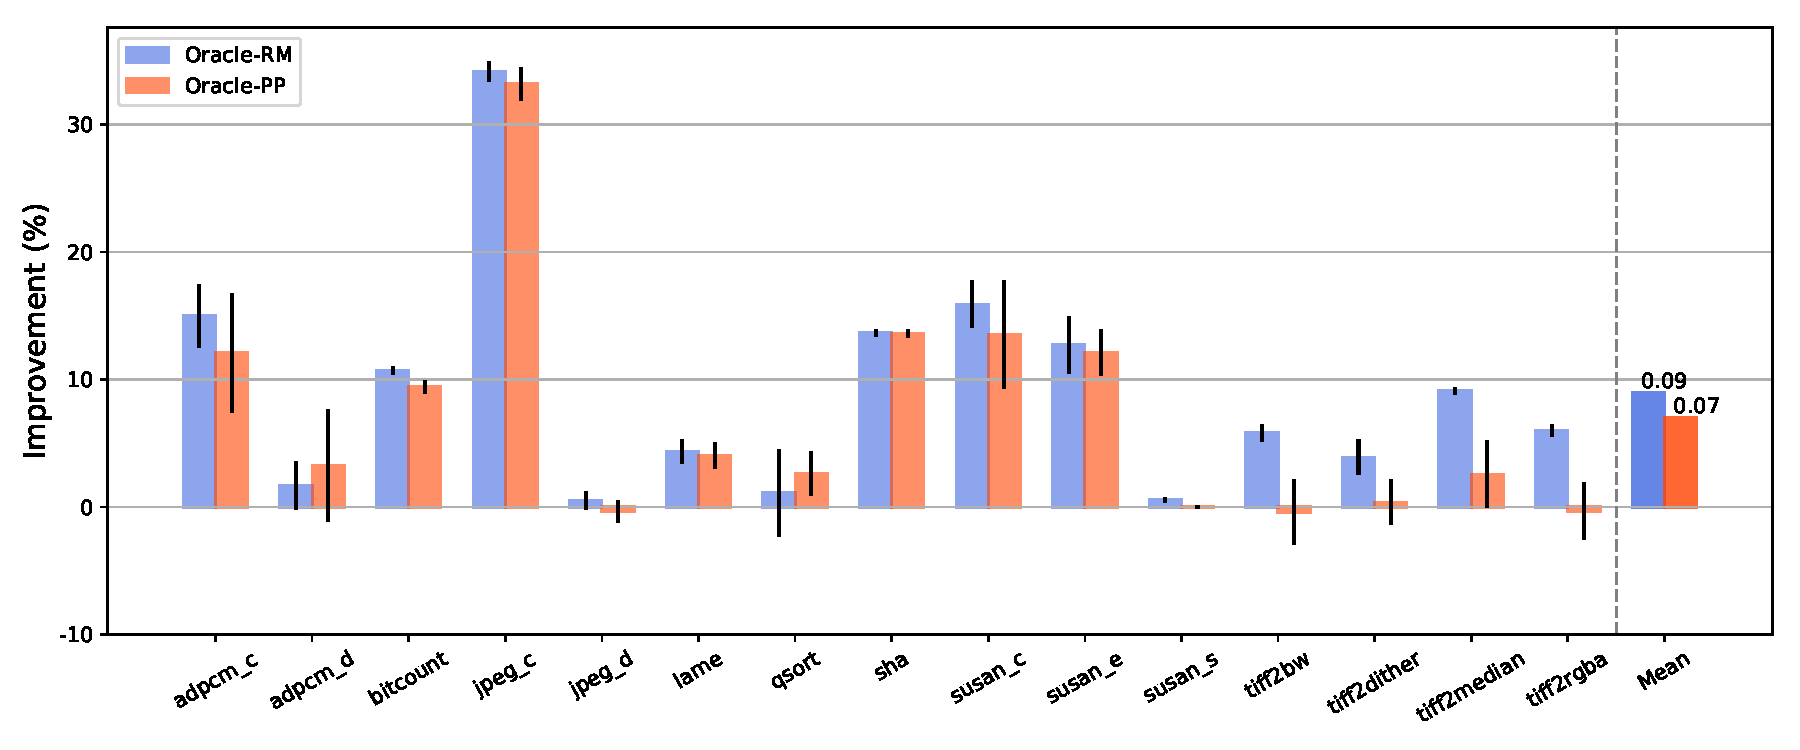
\includegraphics[width=\textwidth]{figs/speedups.pdf}
    \caption{Speedups obtained from the final optimisation sequence selected by the online {\itercomp}.
	         The speedups reported for each benchmark represents the average speedup across their complete 1000 input datasets.}
    \label{fig:speedups}
\end{figure*}

\begin{figure*}[h]
    \centering
    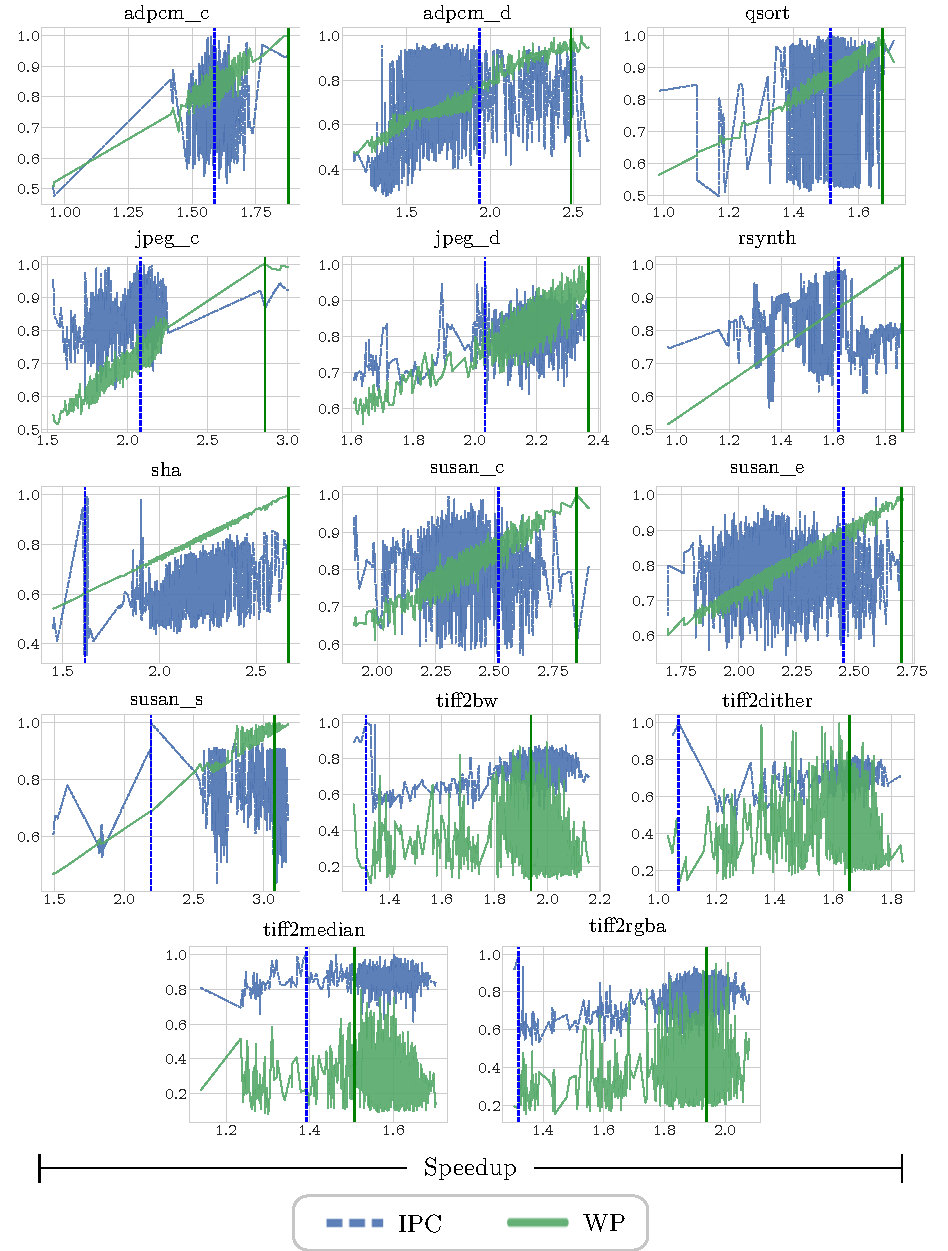
\includegraphics[width=\textwidth]{figs/ipc-vs-work.pdf}
    \caption{Comparison between {\itercomp} using IPC or the WP metric.}
    \label{fig:ipc-vs-work}
\end{figure*}

Figure~\ref{fig:ipc-vs-work} presents a comparison between IPC and the WP metric regarding their correlation with the actual speedup over \verb|-O0| observed during {\itercomp}.
Each point in the figure corresponds to each metric averaged over input windows collected during multiple executions of the {\itercomp}.
The vertical lines correspond to the optimisation sequence selected by the {\itercomp} search, which either represents the highest IPC or the highest value of WP.
In all cases, the optimisation sequence selected based on the WP is much closer to the best speedup than the optimisation sequence selected based on IPC, which can be attributed to the fact that the WP has a stronger correlation with the speedup.
In all cases, IPC shows little to no correlation with the speedup, which corroborates the argument given in Section~\ref{sec:ipc-vs-work-metric}.

For some cases, namely for the tiff-related benchmarks, the WP shows a worse correlation with speedup.
We believe these cases could be improved by improving the cost model used to compute the work metric.
However, even in these cases, the optimisation sequences selected based on the WP outperform those selected based on the IPC metric.

\section{Related Work}

\subsection{{\IterComp}}

Chen~\etal~\cite{chen10,chen12a} evaluate the effectiveness of iterative compilations across a large number of input test cases.
Their main motivation is to answer the question:
\textit{How data input dependent is {\itercomp}?}
Their results show that it is possible to find a combination of compiler optimisations that achieves at least 86\% of the maximum speedup across all input test cases.
These optimal combinations are program-specific and yield average speedups up to 3.75$\times$ over the highest optimisation level of compilers.

When optimising a program, the main method for {\itercomp} used by Chen~\etal~\cite{chen10,chen12a} evaluates each combination of compiler optimisations across all the available inputs, i.e., if $N$ is the number of input test cases and $M$ is the total number of combinations of compiler optimisations, they perform a total of $O(NM)$ runs of the program being optimised.
Furthermore, they use a pre-defined set of only 300 different combinations of compiler optimisations, which represents a very small sample of the optimisation search space for most modern compilers, e.g.
LLVM has 56 distinct optimisation passes and GCC has about 47 high-level (SSA form) optimisation passes and about 25 low-level (RTL) optimisation passes, which in both cases result in much more than $2^{50}$ distinct combinations of compiler optimisations, without considering repetition.

Recent work~\cite{chen12b,fang15} have applied the same idea of performing input-dependent {\itercomp} to distributed applications on data centres.
In summary, each worker receives a subset of the input dataset, called the evaluation dataset, to perform an \textit{online} {\itercomp} of the code being executed.
Each worker performs the same the method for {\itercomp} used by Chen~\etal~\cite{chen10,chen12a}, i.e., they evaluate each combination of compiler optimisations across all the evaluation dataset.
However, because the optimisation is performed online, they usually consider a small evaluation dataset and a small number of compiler optimisations.

Fursin~\etal~\cite{fursin07} addressed the problem of comparing the effect of two optimisations on two distinct inputs. For that purpose, they proposed to use instruction per cycle (IPC) as the metric for performing such comparison.
Their result show that using IPC seems promising as a robust metric for {\itercomp} across large input datasets.
However, some specific optimisation techniques may affect the use of IPC as a robust metric, and specially IPC has been shown to provide poor performance estimation for multi-threaded programs~\cite{alameldeen06,eyerman08}.
In particular, IPC can give a skewed performance measure if threads spend time in \textit{spin-lock loops} or other synchronisation mechanisms. 
Some existing work on performance assessment suggest that total execution time should be used for measuring performance of multi-threaded programs~\cite{alameldeen06,eyerman08}.
Aalameldeen and Wood~\cite{alameldeen06} in particular suggest that a simple work-related metric should be used if the unit of work is representative enough.
Work-related metrics have already been largely used for measuring performance of throughput-oriented applications, for other applications, however, choosing an appropriate unit of work can be more challenging~\cite{alameldeen06}.

\subsection{Work and Input Size Metrics}

Previous work have proposed profiling-based mechanism to estimate input sizes~\cite{zaparanuks12,coppa14}.
Coppa~\etal~\cite{coppa14} in particular propose the concept of \textit{read memory size} for automatically estimating the size of the input passed to a routine, where \textit{read memory size} represents the number of distinct memory cells first accessed by a read operation.
In other words, the \textit{read memory size} metric measures the size of the useful portion of the input's memory footprint.
However, because we are interested in the amount of computational work performed in respect of a given input, the memory footprint of the input may not always have a direct correspondence to  the amount of computational work.

Goldsmith~\etal~\cite{goldsmith07} use \textit{block frequency} as the measure for performance for empirically describing the asymptotic behaviour of programs, which is known as empirical computational complexity.
Block frequency is a relative metric that represents the number of times a basic block executes~\cite{ball94,ball96}.
They argue in favour of block frequency due to its portability, repeatability and exactness, since it does not suffer from timer resolution problems or non-deterministic noises.
Block frequency also has the advantage of being efficiently profiled by means of automatic code instrumentation~\cite{knuth73,ball94}.

However, in the context of comparing different optimisations, although block frequency would be able to capture aspects of optimisations that simplify the control-flow graph (CFG), measuring work at the basic block resolution would not capture effects of optimisations at the instruction level.
Because of that, we extend the idea of using basic block frequency to measure computational work by also considering the computational cost of each basic block.
The computational cost of a basic block is given by weighing the instructions that it contains.

\subsection{Optimal Instrumentation}

In 1973, Donald Knuth~\cite{knuth73} provided an optimal algorithm for profiling block frequency, inserting fewer probes than the previously described naive instrumentation that was commonly used in practice~\cite{knuth71}.
Forman~\cite{forman81} proposed further overhead reductions by placing the probes in basic blocks that are less likely to be executed based on static heuristics.

Ball and Larus~\cite{ball94} offered a detailed discussion comparing two approaches for optimally profiling block frequency, namely, placing probes on the vertices or the edges of the control-flow graph (CFG).
They show that the edge-based approach produces optimal placement of probes.

\section{Conclusion and Future Work}

Our proposed technique for relaxed instrumentation can also be applied for similar profiling scenarios, such as profiling empirical computational complexity~\cite{goldsmith07,zaparanuks12,coppa14}.

\section*{Acknowledgments}

This work was supported by the UK Engineering
and Physical Sciences Research Council (EPSRC) under grants
EP/L01503X/1 for the University of Edinburgh, School
of Informatics, Centre for Doctoral Training in Pervasive
Parallelism, % (\url{http://pervasiveparallelism.inf.ed.ac.uk/}),
and also by the Institute for Computing Systems Architecture (ICSA)
in the School of Informatics at the University of Edinburgh.

\bibliographystyle{ACM-Reference-Format}
\bibliography{bibliography} 

\end{document}
